\clearpage

\section{General Architecture of the Application}

This section outlines the general architecture of the application. It includes the physical architecture and the operation of the architecture.

\subsection{Physical Architecture}

\begin{figure}[ht]
	\centering
	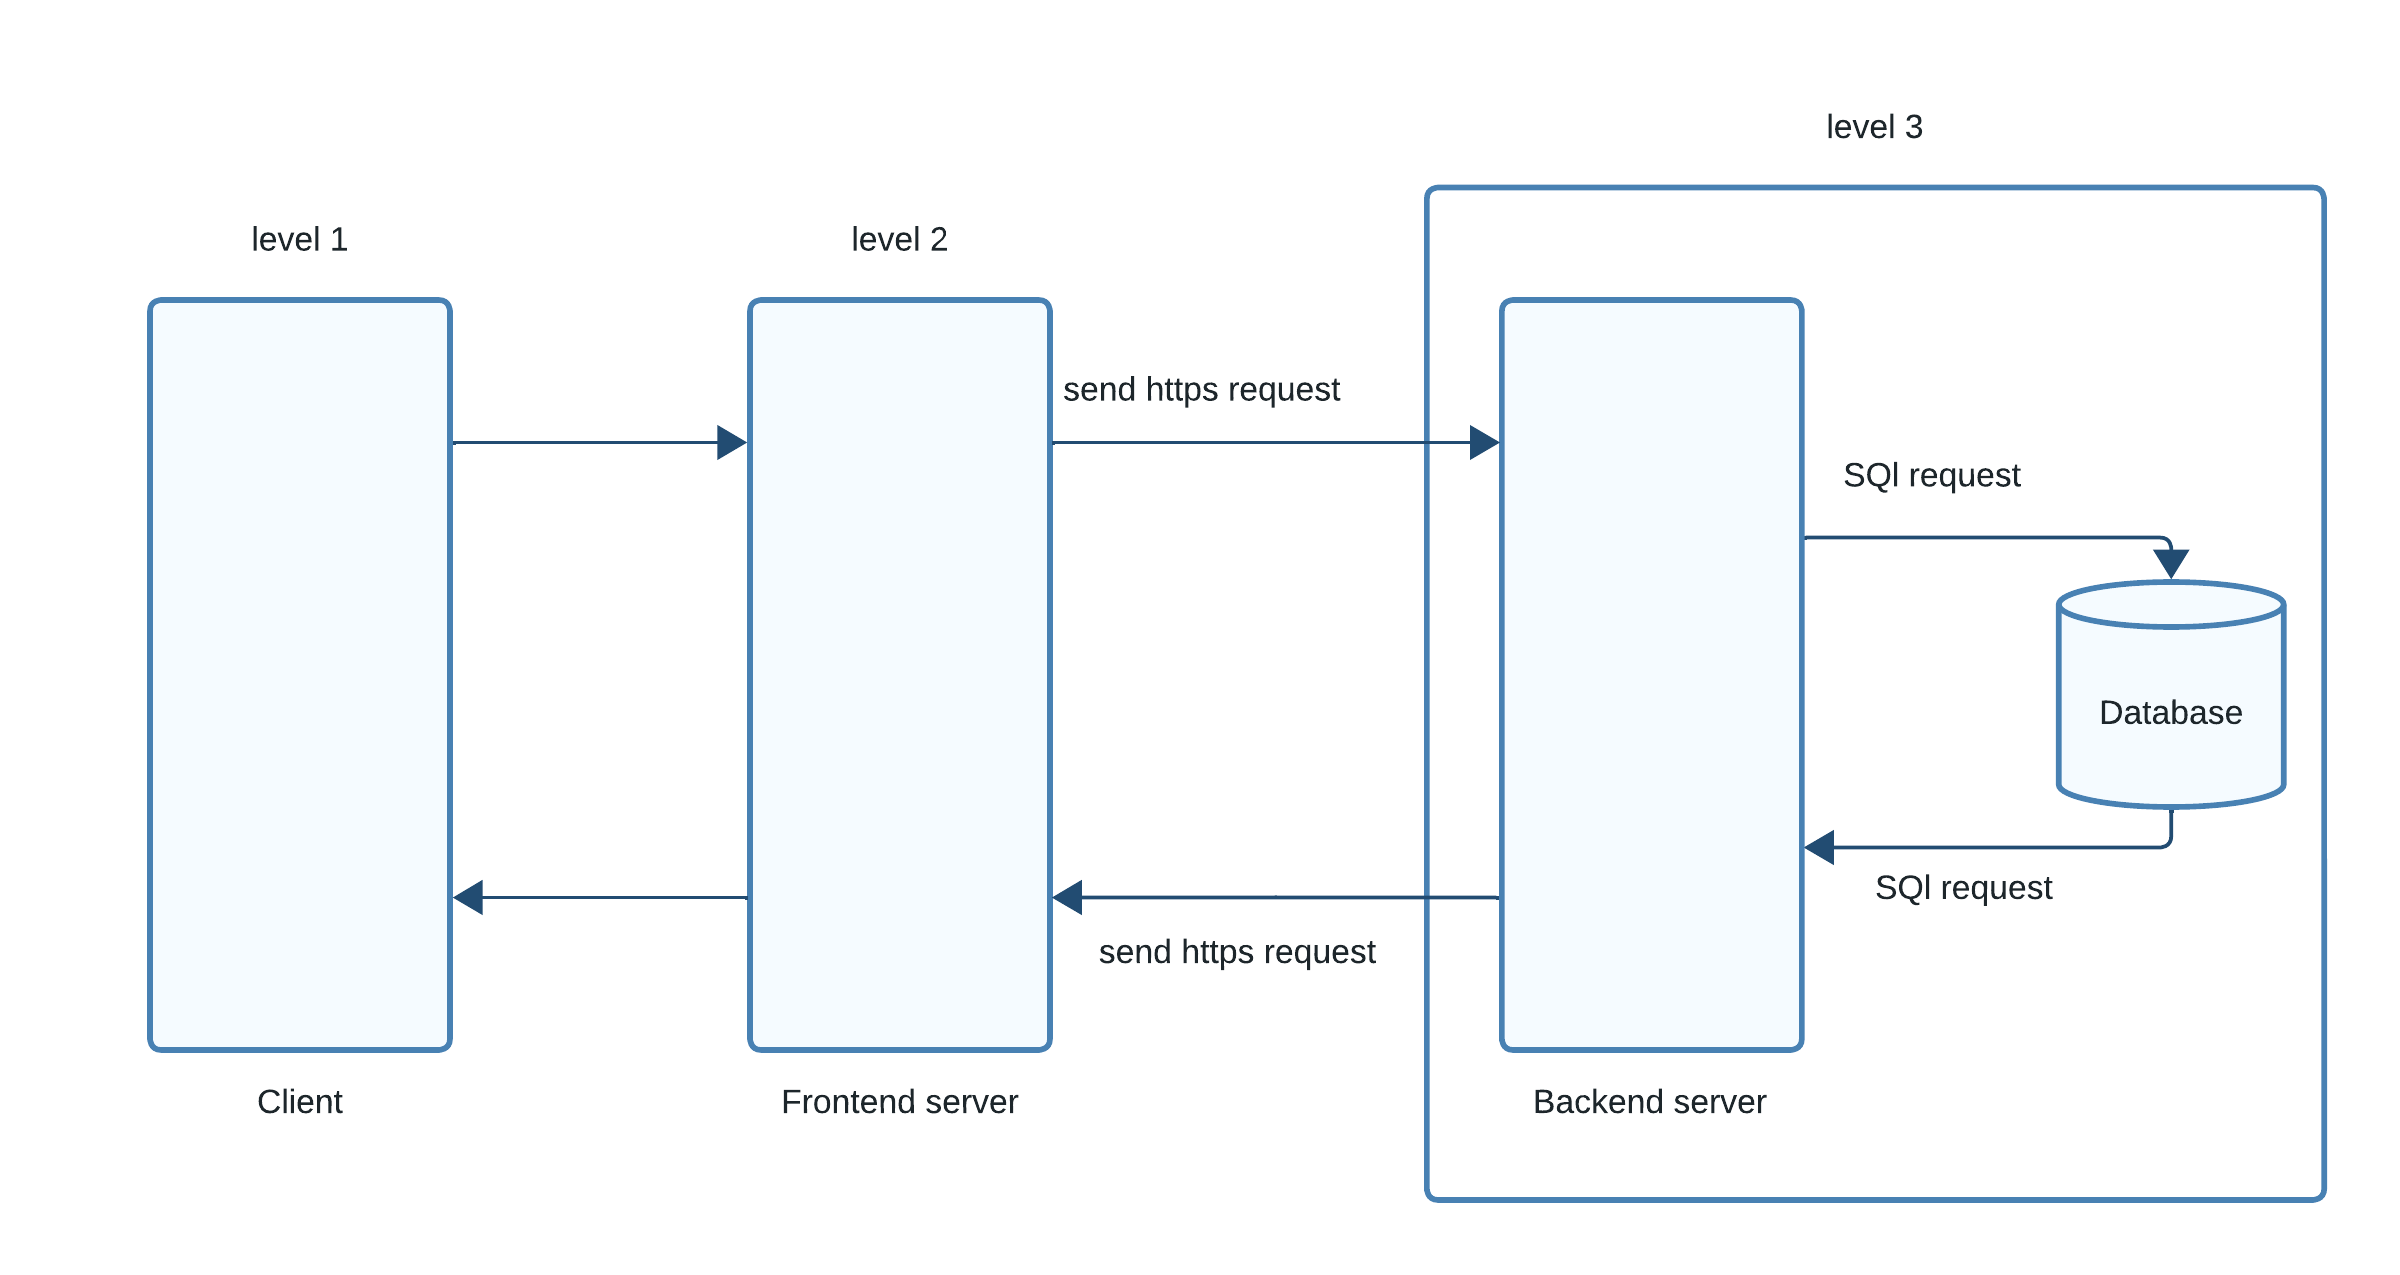
\includegraphics[width=\linewidth]{Images//images/3-tier architecture.png}
	\caption{Global Use Case Diagram}
	\label{fig:Global Use Case Diagram}
\end{figure}

In the physical architecture, I followed the 3-tier architecture:

\begin{itemize}
	\item Level 1 is the Client (Presentation Tier): This is where the user interacts with the system. It could be any user interface like a web page, desktop application, or mobile app.
	\item Level 2 is the Front Server (Application Tier): This is where all the business logic resides. It processes client requests, manages business rules, and controls application functionality.
	\item Level 3 is the Back Server and Database (Data Tier): This is where data is stored and retrieved. It includes the database management system and the servers that manage it.
\end{itemize}

\clearpage
\subsection{Logical Architecture}

\begin{figure}[ht]
	\centering
	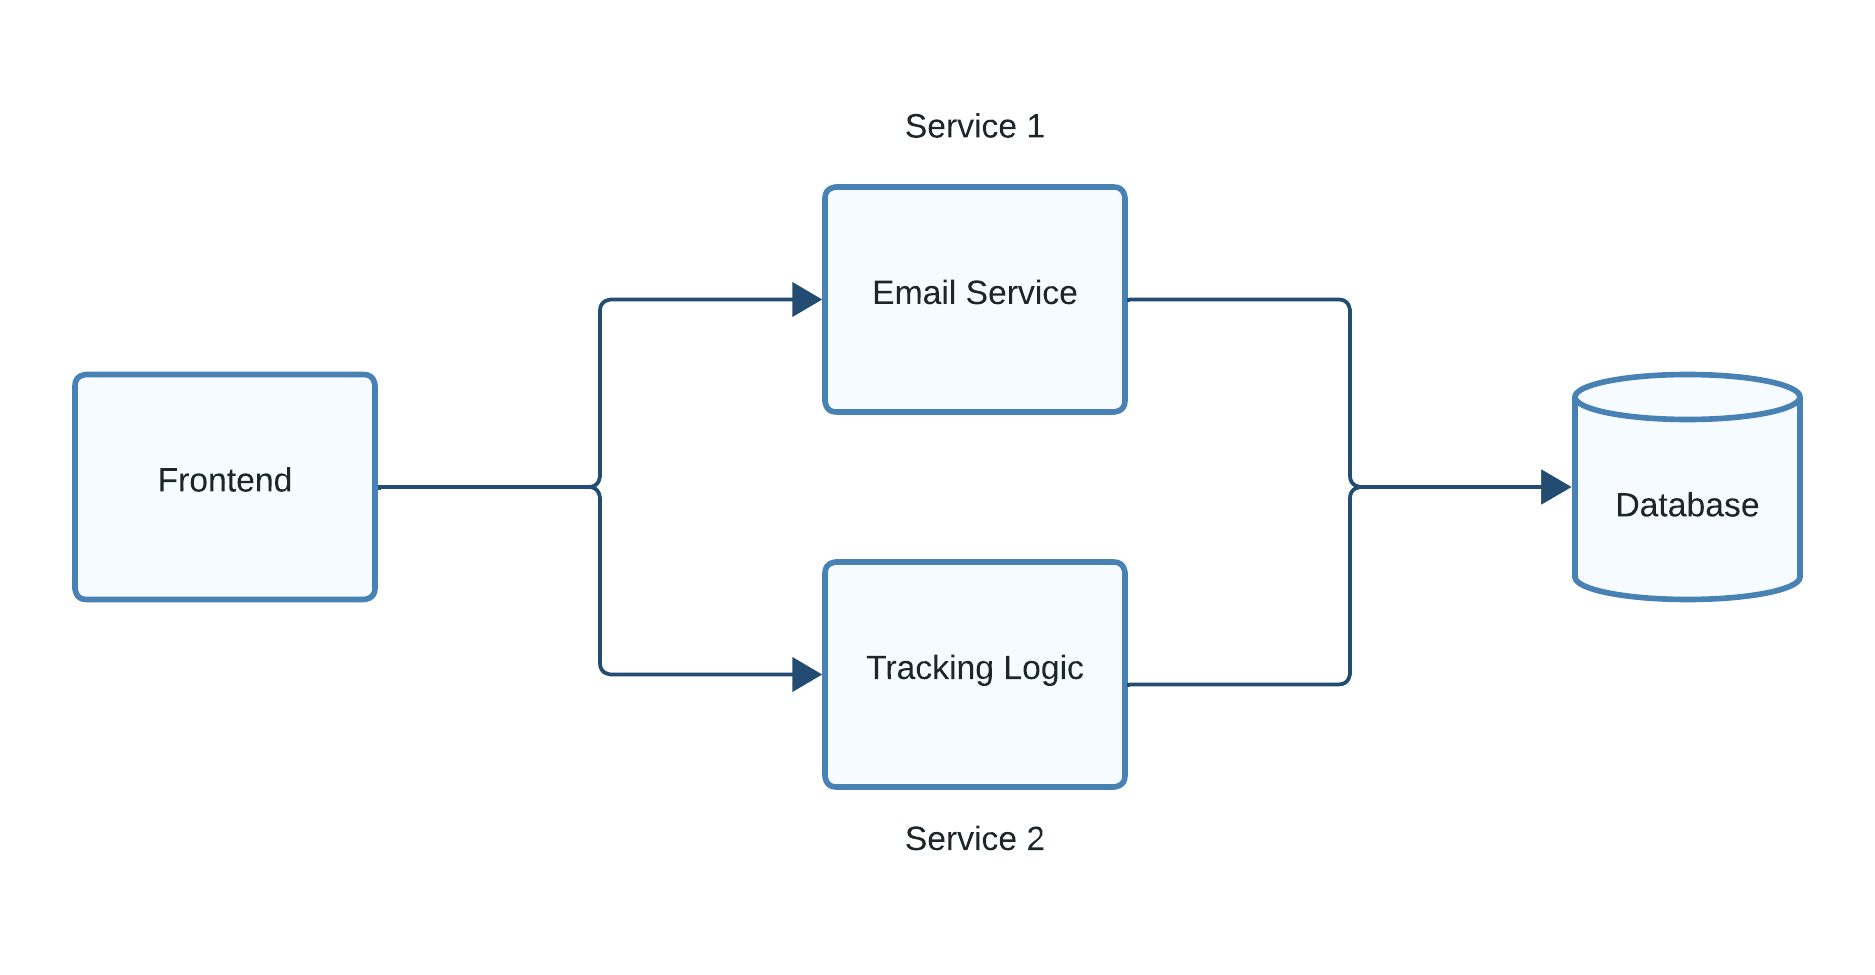
\includegraphics[width=\linewidth]{Images//images/Microservices architechture.png}
	\caption{Global Use Case Diagram}
	\label{fig:Global Use Case Diagram}
\end{figure}
The logical architecture of our email marketing tool consists of several interconnected components:

\begin{itemize}
	\item \textbf{Frontend}:
	      \begin{itemize}
		      \item This component represents the user-facing part of our application.
		      \item It is deployed on Vercel, a platform for hosting frontend applications.
		      \item Users interact with the frontend to create and manage email campaigns, templates, and other settings.
	      \end{itemize}

	\item \textbf{Email Building and Sending Service}:
	      \begin{itemize}
		      \item Responsible for email composition, rendering, and sending logic.
		      \item Communicates with the frontend to receive email content and recipient lists.
		      \item Handles the process of sending emails to recipients.
		      \item It is deployed on Azure.
	      \end{itemize}

	\item \textbf{Tracking Service}:
	      \begin{itemize}
		      \item Tracks email campaign performance metrics.
		      \item Collects data on email opens, clicks, and other relevant events.
		      \item Stores tracking data for analytics and reporting purposes.
              \item It is deployed on Azure.
	      \end{itemize}

	\item \textbf{Database}:
	      \begin{itemize}
		      \item Hosts our Campaign-related data.
		      \item Contains three main tables:
		            \begin{itemize}
			            \item \textbf{Email Campaigns Data}: Stores email content, and recipient information.
			            \item \textbf{Email Template}: Stores built email templates
			            \item \textbf{Tracking Data}: Stores tracking events (e.g., opens, clicks) associated with email campaigns.
		            \end{itemize}
	      \end{itemize}
\end{itemize}
